\section{Trigonometria no Triângulo Retângulo}

\begin{definition}
\label{def:seno-cosseno}
Em um triângulo retânglulo $ABC$, como na Imagem~\ref{fig:triangulo-retangulo}, definem-se o
\textdef{cosseno} ($\cos$) e o \textdef{seno} ($\sen$) dos ângulos agudos do
triângulo:
%
\begin{figure}
\centering
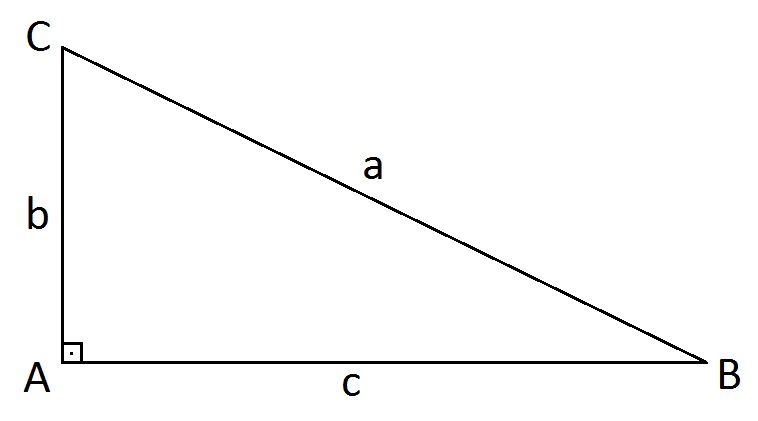
\includegraphics[width=4.8cm]{\imgdirfromsection/triangret.jpg}
\caption{Triângulo retângulo qualquer.}
\label{fig:triangulo-retangulo}
\end{figure}
%
$$\cos \widehat B = \frac c a = \frac {\text{cateto
adjacente}}{hipotenusa}, \ \ \ \ \sen \widehat B = \frac b a = \frac
{\text{cateto oposto}}{hipotenusa},$$
$$\cos \widehat C = \frac b a \ \ \ \ \text{e} \ \ \ \ \sen \widehat
C = \frac c a.$$    
\end{definition}

\begin{remark}
As relações definidas como o foram na Definição~\ref{def:seno-cosseno} são únicas para cada ângulo em
decorrência da proporcionalidade dos lados de triângulos
semelhantes. Portanto, calculam-se o seno e o cosseno de um ângulo
independentemente do triângulo retângulo que o contém.
\end{remark}

\begin{proposition}
    \begin{itemize}
\item O cosseno de um ângulo agudo é igual ao seno do seu
complementar e vice-versa, e é daí que surgiu o termo ``cosseno'' (seno do
complemento);
\item O seno e o cosseno são números compreendidos entre 0 e 1 por
serem razões entre um cateto pela hipotenusa de um triângulo
retângulo.
\end{itemize}
\end{proposition}

\begin{proposition}[Relação Fundamental da Trigonometria]
Seja $\widehat B$ um dos ângulos agudos de um triângulo retângulo
cuja hipotenusa mede $a$ e os catetos, $b$ e $c$. Então:
$$\sen^2 \widehat B + \cos^2 \widehat B = 1.$$
\end{proposition}

\begin{onlineact}
    \khan{https://pt.khanacademy.org/math/trigonometry/trigonometry-right-triangles/intro-to-the-trig-ratios/e/trigonometry_1}
    {Razões Trigonométricas em Triângulos
Retângulos}.
\end{onlineact}

\begin{onlineact}
    \khan{https://pt.khanacademy.org/math/trigonometry/trigonometry-right-triangles/trig-solve-for-a-side/e/trigonometry_2}
    {Atividade 20 - Como Calcular a Medida de um Lado em Triângulos
Retângulos}.
\end{onlineact}